\def\year{2016}
%File: formatting-instruction.tex
\documentclass[letterpaper]{article}
%\usepackage{aaai}
%\usepackage{times}
%\usepackage{helvet}
%\usepackage{courier}
%\usepackage{amsfonts}
\usepackage{amsmath}
\usepackage{amssymb}
%\usepackage{color}
\usepackage{graphicx}
%\usepackage{subfigure}
%\graphicspath{{figs/}}
%\frenchspacing
%\setlength{\pdfpagewidth}{8.5in}
%\setlength{\pdfpageheight}{11in}
%\setcounter{secnumdepth}{0}  
 \begin{document}
% The file aaai.sty is the style file for AAAI Press 
% proceedings, working notes, and technical reports.
%
\title{Twitter Project: White Paper}
\author{F. M. Delle Fave
%Association for the Advancement of Artificial Intelligence\\
%2275 East Bayshore Road, Suite 160\\
%Palo Alto, California 94303\\
}
\maketitle

\section{Problem Description}

From a high-level perspective the aim of this work is to make sense of twitter data. Specifically, we aim to extract information from tweets, and use such information to measure similarity between tweets. Our scope is general, we wish to capture all types of information--- the topic of a tweet, the sentiments of the user posting the tweet or the relevance of a tweet to some specific question--- and use it to define the best possible similarity, or distance, measure between tweets.

There exists a vast literature about measuring similarity between words, sentences, paragraphs and general documents. The key idea, is to transform a sequence of words into a vector representation within a vector space and then use standard distance metrics, such as euclidean or cosine distance to define their similarity. Cosine similarity, in particular, has been shown to characterize well the semantic similarity between sequences of words. In essence, the cosine similarity of two vectors $v_1$ and $v_2$ varies within a spectrum of values going from $0$, in which case the two vectors are orthogonal (i.e., no semantic similarity at all) to $v_1 \cdot v_2 = v^2$ in which case the two vectors are parallel (same semantics). 

In this work, we aim to define a novel similarity metric which work specifically for measuring semantic similarity between tweets. To be specific, we wish to learn such metric using semi-supervised data. In what follows, we describe our initial model and key ideas about the key research challenges of this work, and on how we wish to proceed from now on. 

\section{Problem Model}

We consider a set of tweets $\mathcal{T} = \{ t_1, t_2, t_3, \dots, t_M \}$, where $M$ can be as large as several millions. Given this data, we wish two learn: (i) the word representation of a tweet and (ii) a distance metric between tweets based on this representation. We first describe how we define our word representation and then we describe the metric learning problem.

\subsection{Word Representations for Tweets}

We wish to define a word representation $\mathbf{x}_t$ for each tweet $t \in \mathcal{T}$. Ideally, we could use one of the existing word2vec models, which calculate a vector representation by counting word n-gram frequencies and calculating the probability that a specific sequence of word will appear together within a specific set of documents \cite{Mikolov2013a}. By doing so, however, we would consider each word within a tweet to have the same importance as the other ones. 

In information retrieval applications, this is not recommended. To understand the context, or the semantics, of tweets, some keywords will matter more than others and this importance need to be reflected in the vector representation of a specific tweet. For instance, if a twitter user talks about a specific movie in either a positive or negative way, all keywords referring to the movie or about the user's sentiment about it need to be emphasized.  To achieve this type of representation, in our work, we build upon CBOW \cite{Mikolov2013a}, and upon the model described in \cite{Ling2015a}, to define our own representation: 

\begin{equation}
\mathbf{x}_t  = \sum_{w_i \in t} \mathcal{I}(w_i) \cdot \mathbf{x}_i 
\label{eq:sum_of_words}
\end{equation}
where $\mathbf{x}_t$ is the representation of tweet $t$, $\mathbf{x}_i$ is the representation of word $w_i$ in tweet $t$ and, most importantly, $\mathcal{I}(w_i)$ is the importance of word $w_i$\footnote{note: notation suggests that this is a function which is not the case here...}.  

In our work, we are specifically interested in defining the function $\mathcal{I}$. Initially, we will consider some simple cases such as constant functions, e.g., $\mathcal{I}(w_i) = 1$ or $\mathcal{I}(w_i) = \frac{1}{|t|}$. Next, we plan to define this function such that it learns all the different pieces of information that we wish to extract from a tweet, e.g., relevance, sentiment, topic, \emph{etc}.  One simple example of a function could be $\mathcal{I}(w_i) = c_{r} (w_i) \cdot c_{a} (w_i) \cdot c_{s} (w_i)$, where $c_{r}$, $c_{a}$ and $c_{s}$ are well-defined coefficients leveraging, respectively, the relevance, the topic and the sentiment of word $ w_i$ in tweet $t$. 

One interesting aspect of function $\mathcal{I}$ is that it transforms the original problem of learning a word representation into a multi-task learning problem, whereby each task is a piece of information that we wish to extract from a tweet, as discussed above. With this new function then, we need to define a new type of distance function that uses the information provided by each task to improve its accuracy.  

\subsection{Multi-Task Distance Function for Tweets}

We want to learn a distance function between word representations of tweets, as discussed in the previous section, and, potentially of any type of sequences of words (e.g., keywords, queries, sentences, \emph{etc}...). Formally, we define the distance metric as $d(\mathbf{x}_t, \mathbf{x}_s)$ where $\mathbf{x}_t$ and $\mathbf{x}_s$ are word representations of respectively a tweet $t$ and a sequence of words $s$. One possible application of this metric is information retrieval. Data analytics teams often need to mine very large datasets, looking for tweets about specific topics, reflecting a specific sentiment, or relevant to a specific query. These retrieval tasks are typically solved by searching for well-defined key-words within the tweets. However, a more sophisticated type of search, which understands the context of a specific tweet, could be much more accurate for this 
type of semantic queries. 

In this work, we take inspiration from \cite{Parameswaran2010a} and define the distance function for a specific task $s, r$ or $a$ as the Mahalanobis distance between the two vector representations: 
\begin{align}
d_{s} (\mathbf{x}_t, \mathbf{x}) &= \sqrt{  (\mathbf{x}_t - \mathbf{x})^{\intercal}\ (\mathbf{W}_0 + \mathbf{W}_s)\ (\mathbf{x}_t - \mathbf{x})}\label{eq:dist-1}\\
d_{r} (\mathbf{x}_t, \mathbf{x}) &= \sqrt{  (\mathbf{x}_t - \mathbf{x})^{\intercal}\ (\mathbf{W}_0 + \mathbf{W}_r)\ (\mathbf{x}_t - \mathbf{x})}\label{eq:dist-2}\\
d_{a} (\mathbf{x}_t, \mathbf{x}) &= \sqrt{  (\mathbf{x}_t - \mathbf{x})^{\intercal}\ (\mathbf{W}_0 + \mathbf{W}_a)\ (\mathbf{x}_t - \mathbf{x})}\label{eq:dist-3}
\end{align}
where each of the matrices $\mathbf{W}_0$, $\mathbf{W}_s$, $\mathbf{W}_r$ and $\mathbf{W}_a$ is positive semi-definite and has the same meaning as in \cite{Parameswaran2010a}, i.e., $\mathbf{W}_0$ picks up general trends across the entire dataset $\mathcal{T}$, whereas $\mathbf{W}_s$, $\mathbf{W}_r$ and $\mathbf{W}_a$ pick up trends pertaining to each specific task.  

Given the three distances above, and a specific tweet $t$, we can define the optimization problem that we wish to solve as follows: 
{\footnotesize
\begin{align}
&\min_{\mathbf{W}_0, \mathbf{W}_s, \mathbf{W}_r, \mathbf{W}_a} \gamma_0 || \mathbf{W}_0 - \mathbf{I}||^2_F + \sum_{l \in \{s, r, a\}} \left[  \gamma_l || \mathbf{W}_l ||^2_F + \sum d_{l}^2 ( \mathbf{x}_t, \mathbf{x} ) + \sum_{(t,j,k) \in S_l} \xi_{tjk} \right]\\
&\quad \quad \mathbf{subject\ to:}\ \forall l \in \{ s, r, a\}, \forall (t, j, k) \in S_l: \\
& \quad \quad \quad \quad d^2_l ( \mathbf{x}_t,  \mathbf{x}_j) - d^2_l ( \mathbf{x}_t,  \mathbf{x}_j) \leq 1 - \xi_{tjk}\\ 
& \quad \quad \quad \quad \xi_{tjk} \geq 0\\
& \quad \quad \quad \quad \mathbf{W}_0, \mathbf{W}_s, \mathbf{W}_r, \mathbf{W}_a \succeq	0
\end{align}
}
One important difference with \cite{Parameswaran2010a} is that twitter data is unsupervised, and is often very large. This means that: (i) we do not have a predefined dataset of neighbors, (ii) calculating this dataset for \emph{all} instances is practically impossible and, finally (iii) the optimization problem defined above, as acknowledged by the authors in \cite{Parameswaran2010a} will not scale to datasets with more than 10000 instances.  These are the three research challenges that we will try to address in this work. Specifically, (i) and (ii) will require some form of active learning, which will be discussed later. Then, we aim to solve the third challenge by using a neural network representation of the problem. Our initial ideas to address this challenge are discussed next.

\section{A Neural Network Representation for learning Mahalanobis Distance}

\begin{figure}
\centering
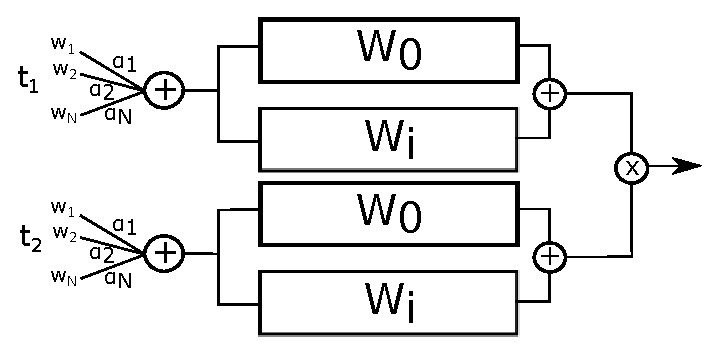
\includegraphics[width=0.7\linewidth]{figures/siamese_1}
\label{fig:siamese_1}
\caption{The architecture of a siamese network}
\end{figure}

Our objective is to define a neural network architecture that can learn equations \ref{eq:dist-1}, \ref{eq:dist-2} and \ref{eq:dist-3}, which we summarize below: 
\begin{equation}
\forall i \in \{s, t, o\}\  d_i(\mathbf{x}_t, \mathbf{x}) = \sqrt{( \mathbf{x}_t - \mathbf{x})^\intercal(\mathbf{W}_0 + \mathbf{W}_i) ( \mathbf{x}_t - \mathbf{x})}\label{eq:mahalanobis-dist} 
\end{equation}
In essence, this job consists of learning the Mahalanobis matrix $\mathbf{W} = \mathbf{W}_0 + \mathbf{W}_i$, which can be done by adapting a siamese network, a well known type of neural network representation used in computer vision \cite{Chopra2005a, Zagoryuko2015}, to the setting being studied here. The architecture is described in Figure \ref{fig:siamese_1}.  To understand how it works, we can think of it as a pipeline, which proceeds in three phases.  

First, a weighted average of two tweets is calculated: 
\begin{align}
\mathbf{x}_{t_1} &= \sum^N_{i =1} \alpha^1_i x_{w^1_i}\\
\mathbf{x}_{t_2} &= \sum^N_{i =1} \alpha^2_i x_{w^2_i} 
\end{align}
Note that in our specific case, to follow exactly Equation \ref{eq:mahalanobis-dist}, we should learn the distance between differences of word representations, i.e., $(\mathbf{x}_t - \mathbf{x})$. In what follows, for the sake of clarity, we simplified the description of the architecture, by considering only single word representations. The general architecture is pretty similar to the one in the figure. It simply adds a difference operator to the first layer. 

Second, we learn a linear Neural Network layer based on these two representations: $f(\mathbf{x}_{t_1}) = (\mathbf{W}_0 + \mathbf{W}_i) \mathbf{x}_{t_1}$ and $f(\mathbf{x}_{t_2}) = (\mathbf{W}_0 + \mathbf{W}_i) \mathbf{x}_{t_2}$. One key constraint, here is that the two matrices  $\mathbf{W}_0$ and $\mathbf{W}_i$ need to remain the same for both representations $\mathbf{x}_{t_1}$ and $\mathbf{x}_{t_2}$. This equality constraint needs to be enforced during training. 

The advantage of using a siamese network can be seen in the third phase. Here we multiply the output of the two previous phases and we obtain a positive semi-definite matrix as required by the Mahalanobis distance: 
\begin{align}
f( \mathbf{x}_{t_1}, \mathbf{x}_{t_2} ) &= (\mathbf{W} \mathbf{x}_{t_1})^\intercal (\mathbf{W} \mathbf{x}_{t_2})\\
&= \mathbf{x}^{\intercal}_{t_1} \mathbf{W}^\intercal \mathbf{W} \mathbf{x}_{t_2}\\
&= \mathbf{x}^{\intercal}_{t_1} \mathbf{L} \mathbf{x}_{t_2}
\end{align} 
where $\mathbf{W} = \mathbf{W}_0 + \mathbf{W}_i$ for each specific task $i$ and $\mathbf{L}$ is positive semi-definite since it is the product of two matrices. 

Finally, we describe the cost function used to train this architecture. We define $g(\mathbf{x}_{t_1}, \mathbf{x}_{t_2}) = f(\mathbf{x}_{t_1})^\intercal f(\mathbf{x}_{t_2})$, i.e., the output of the siamese network. The objective of our problem is to minimize the following loss function: 
\begin{equation}
\max (0, m - h(\mathbf{x}_{t_1}, \mathbf{x}_{t_2}, \mathbf{x}_{t_3}) )
\label{eq:loss}
\end{equation}
where $m$ is a slack variable to account for noise in the data and h is a function which calculates the distance between positive and negative examples: 
\begin{equation}
h(\mathbf{x}_{t_1}, \mathbf{x}_{t_2}, \mathbf{x}_{t_3}) = g(\mathbf{x}_{t_1}, \mathbf{x}_{t_2}) - g(\mathbf{x}_{t_1}, \mathbf{x}_{t_3}) 
\end{equation}
where $t_1$ and $t_2$ are positive examples, in the sense that they are close between each other, and $t_3$ is a negative example because it is far from $t_1$. 

Hence, to use the architecture in Figure \ref{fig:siamese_1}, one need to solve Equation \ref{eq:loss} for both positive and negative examples. To achieve this, we will use Amazon Mechanical Turk. Our idea is to implement an active learning routine, where iteratively: (i) we ask workers on Mechanical Turk to determine positive and negative examples and (ii) we use these examples to calculate our new representation and repeat until we are satisfied with the result. 

\bibliography{bibliography}
\bibliographystyle{plain}

\end{document}